
\documentclass[aspectratio=169]{beamer}

% Copyright (C) 2012 - EDF R&D - Michael Baudin

% To highlight source code
\usepackage{listings}
\definecolor{darkgreen}{rgb}{0,0.5,0}
\definecolor{violet}{rgb}{0.5,0,1}

% \usepackage{lmodern}% http://ctan.org/pkg/lm

\usetheme{Darmstadt} % http://tex.stackexchange.com/questions/177042/beamer-latex-customized-formats

\useoutertheme[subsection=false,footline=authortitle]{miniframes}
% RGB scaled on 0-255 scale (section 17.1.1), colors pulled from title block
\usecolortheme[RGB={44, 131, 82}]{structure}

% hide header:
\setbeamertemplate{headline}{}

\usepackage[utf8]{inputenc}
\usepackage[T1]{fontenc}

%\usepackage[french]{babel}
%\uselanguage{French}
%\languagepath{French}

\def\bx{{\bf x}}
\def\RR{\mathbb{R}}

% The physical model
\newcommand{\model}{g}
\newcommand{\inputDim}{d}  % The input dimension of the model
\newcommand{\outputDim}{{d_Y}}  % The output dimension of the model
\newcommand{\metaModel}{\widetilde{\model}}  % The surrogate model

% Probabilistic modeling
\newcommand{\inputRV}{\vect{X}}  % The input random vector of the model
\newcommand{\outputRV}{\vect{Y}}  % The output random vector of the model
\newcommand{\inputMeasure}{\mu_{\inputRV}}  % The distribution of the input random vector of the model
\newcommand{\outputMeasure}{\mu_{\outputRV}}  % The distribution of the output random vector of the model
\newcommand{\standardRV}{\vect{Z}}  % The standard random vector (e.g. for polynomial chaos expansion)
\newcommand{\RVU}{\vect{U}}

% For matrixes and vectors
\newcommand{\vect}[1]{{\mathbf{\boldsymbol{{#1}}}}}
\newcommand{\mat}[1]{{\vect{\vect{#1}}}}
\newcommand{\Tr}[1]{{#1}^\top}

% Probabilistic operators
\newcommand{\muX}{\vect{\mu}_{\:X}}
\newcommand{\Var}[1]{{\rm Var}\left( #1 \right)}
\newcommand{\Cov}[1]{{\rm Cov}\left( #1 \right)}
\newcommand{\Expect}[1]{{\mathbb E}\left[ #1 \right]}
\newcommand{\Econd}[2]{{\mathbb E}_{#1}\left[ #2 \right]}
\newcommand{\Prob}[1]{{\mathbb P}\left( #1 \right)}
\newcommand{\ProbCond}[2]{{\mathbb P}_{#1}\left( #2 \right)}
\newcommand{\ech}{\left\{ x_1, \, \dots\,, x_N  \right\}}
\newcommand{\matcov} {\mathbf C}
\newcommand{\matcor} {\mathbf R}
\newcommand{\fcar}[2] {{\mathbf 1}_{#1}(#2)}

\newcommand{\pyvar}[1]{\texttt{#1}}

\def \ot {OpenTURNS}

\hypersetup{colorlinks=true}

\lstset{
  % general command to set parameter(s)
   %basicstyle=\footnotesize\ttfamily, %
   %basicstyle=\normalsize \ttfamily, %
   basicstyle=\scriptsize\ttfamily, %
   keywordstyle=\color{violet}\bfseries,%
   commentstyle=\color{darkgreen}\bfseries,%
   showspaces=false,%
   stringstyle=\color{red}\bfseries, 
   otherkeywords={Gumbel, TruncatedDistribution, LatentVariableModel, %
        SmoothedUniformFactory, Uniform, PythonFunction, JointDistribution, %
        StudentCopula, StudentCopulaFactory, RankSobolSensitivityAlgorithm, %
	   MonteCarlo, IntervalMesher, PointToFieldFunctionalChaosAlgorithm, FieldFunctionalChaosSobolIndices, HistogramFactory, %
	   Graph, BoxCoxFactory, CompositeProcess, WhittleFactory, ARMAFactory, %
	   Basis, TrendFactory, BoxCoxTransform, SpatialFunction, TimeSeries, %
	   WelchFactory, GreaterOrEqual, IndependentCopula, %
	   FunctionalChaosAlgorithm, LowDiscrepancyExperiment, HaltonSequence, LOLAVoronoi,
	   LineSampling, FORM, SafeAndSlow, Brent, Cobyla,
	   SystemFORM, UnionEvent, IntersectionEvent},
}


\title[OpenTURNS]{OpenTURNS release highlights}

\author[OpenTURNS et al.]{J. Schueller (Phimeca)}

\date[]{User Day \#18, June 13th 2025, EDF Lab}

\titlegraphic{
  
\includegraphics[height=0.05\textheight]{figures/airbus-logo.png} \hfill
  
\includegraphics[height=0.09\textheight]{figures/logo-edf.png} \hfill
  
\includegraphics[height=0.09\textheight]{figures/imacs-logo.jpg} \hfill
  
\includegraphics[height=0.05\textheight]{figures/onera-logo.png} \hfill
  
\includegraphics[height=0.08\textheight]{figures/logo-phimeca.png}
  }

%%%%%%%%%%%%%%%%%%%%%%%%%%%%%%%%%%%%%%%%%%%%%%%%%%%%%%%%%%%%%%%%%%%%%%%%%%%%%

  \begin{document}

%%%%%%%%%%%%%%%%%%%%%%%%%%%%%%%%%%%%%%%%%%%%%%%%%%%%%%%%%%%%%%%%%%%%%%%%%%%%%

  \begin{frame}
  \titlepage
  \end{frame}

\begin{frame}
\frametitle{Overview}

New features since last year in releases:

\begin{itemize}
\item v1.24: fall 2024
\item v1.25: spring 2025
\end{itemize}

\end{frame}
  
%%%%%%%%%%%%%%%%%%%%%%%%%%%%%%%%%%%%%%%%%%%%%%%%%%%%%%%%%%%%%%%%%%%%%%%%%%%%%

\begin{frame}
\frametitle{Contents}
\tableofcontents
\end{frame}

%%%%%%%%%%%%%%%%%%%%%%%%%%%%%%%%%%%%%%%%%%%%%%%%%%%%%%%%%%%%%%%%%%%%%%%%%%%%%

\begin{frame}{Not about}

\begin{itemize}
\item New conditional modelling features
\item New quantile estimation features
\item New GP API
\end{itemize}

\end{frame}

%%%%%%%%%%%%%%%%%%%%%%%%%%%%%%%%%%%%%%%%%%%%%%%%%%%%%%%%%%%%%%%%%%%%%%%%%%%%%

\section{Line sampling simulation}

\begin{frame}
\frametitle{Line sampling simulation 1/5}

\begin{block}{Description}

\begin{itemize}
  \item Contract EDF with E. Ardillon, A. Ajenjo, J. Mure with Phimeca

  \item Simulation algorithm comparable to directional sampling
  
  \item Implements the original algorithm from \footnote{Koutsourelakis, H. Pradlwarter, G. Schueller,
\textit{Reliability of structures in high dimensions, part i: algorithms and applications},
Probabilistic Engineering Mechanics 19 (4) (2004) 409–417}
+ adaptive important direction variant from \footnote{Angelis M., Patelli E., Beer M., \textit{Advanced line sampling for efficient robust reliability analysis},
Structural safety, 52 :170-182, 2015.}

  \item The line sampling algorithm estimates the probability of the event $\cD_f$:
  
  $$P_f = \Prob{\model\left( \inputRV \right) \leq 0}
        = \int_{\Rset^{\inputDim}} \mathbf{1}_{\{\model(\vect{x}) \leq 0 \}}\inputMeasure(\vect{x})\di{\vect{x}}$$

\end{itemize}

\end{block}

\end{frame}

%%%%%%%%%%%%%%%%%%%%%%%%%%%%%%%%%%%%%%%%%%%%%%%%%%%%%%%%%%%%%%%%%%%%%%%%%%%%%

\begin{frame}
\frametitle{Line sampling simulation 3/5}

\begin{block}{Algorithm}

The generic line sampling algorithm follows the steps for $k=1, \hdots \sampleSize$:


\begin{itemize}
% 
\item Draw a sample $\vect{z_k} \sim Z$ and project it on the hyperplane normal to $\vect{\alpha}$
  to obtain $P^{\perp}_{\vect{\alpha}}(\vect{z_k})$.

\item Find the roots of $r \mapsto g \circ T^{-1}(r \vect{\alpha} + P^{\perp}_{\vect{\alpha}}(\vect{z_k}))$.

\item Use the roots to compute $p_{\vect{z_k}} = \Prob{R \in I_{P^{\perp}_{\vect{\alpha}}(\vect{z_k})}}$.
% 
\end{itemize}

The global probability $P_f$ is computed from all the $p_{\vect{z_k}}$ probabilities:

$$\widehat{P}_{f,LS} = \frac{1}{\sampleSize} \sum_{i=1}^{\sampleSize} p_{\vect{z_k}}$$

\end{block}

\end{frame}

%%%%%%%%%%%%%%%%%%%%%%%%%%%%%%%%%%%%%%%%%%%%%%%%%%%%%%%%%%%%%%%%%%%%%%%%%%%%%

\begin{frame}
\frametitle{Line sampling simulation 3/5}

\begin{figure}
   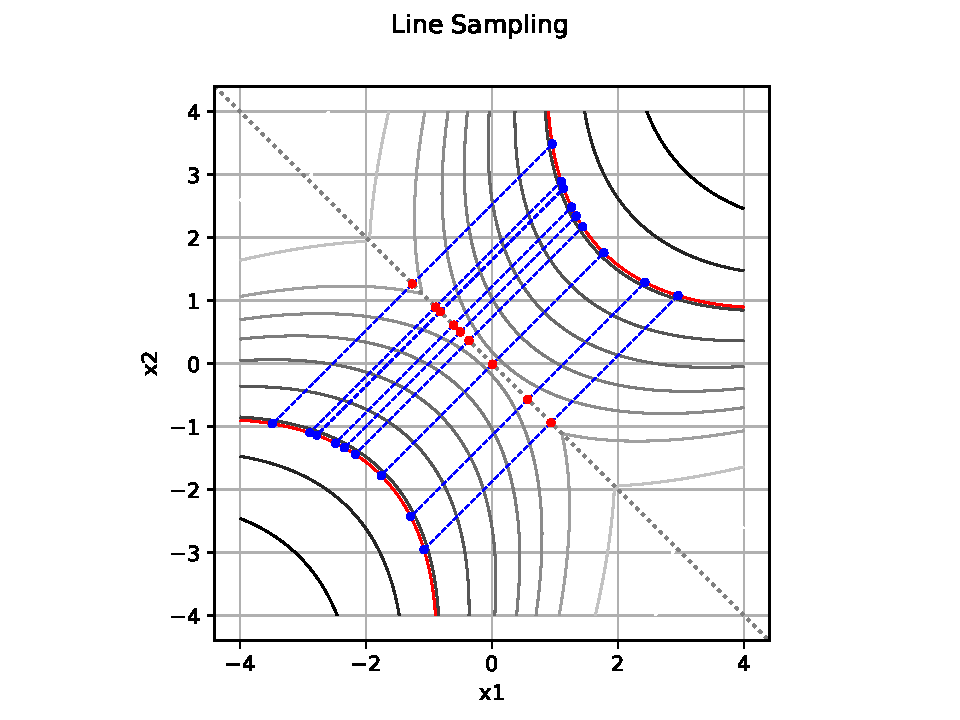
\includegraphics[width=0.7\textwidth]{figures/ls0}
\end{figure}

\end{frame}

%%%%%%%%%%%%%%%%%%%%%%%%%%%%%%%%%%%%%%%%%%%%%%%%%%%%%%%%%%%%%%%%%%%%%%%%%%%%%

\begin{frame}
\frametitle{Line sampling simulation 4/5}

\begin{figure}
   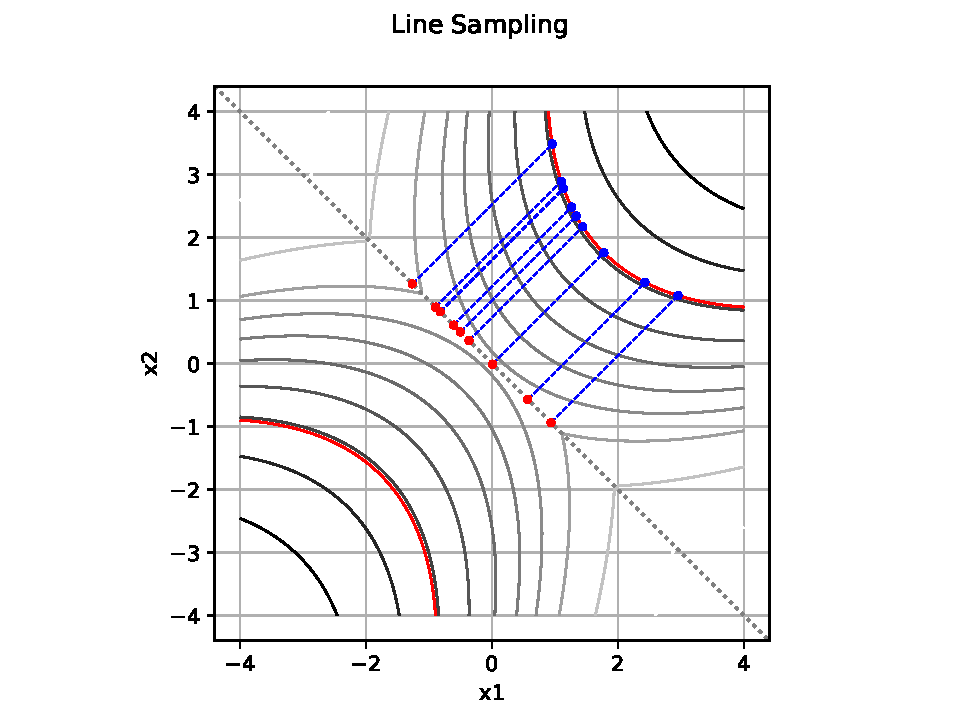
\includegraphics[width=0.7\textwidth]{figures/ls1}
\end{figure}

\end{frame}

%%%%%%%%%%%%%%%%%%%%%%%%%%%%%%%%%%%%%%%%%%%%%%%%%%%%%%%%%%%%%%%%%%%%%%%%%%%%%

\begin{frame}[containsverbatim]
\frametitle{Line sampling simulation 5/5}

\begin{small}
\lstset{language=python}
\begin{lstlisting}
# 1. preliminary FORM
optim = ot.Cobyla()
optim.setStartingPoint(X.getMean())
algo = ot.FORM(optim, event)
algo.run()
result_form = algo.getResult()
alpha = result_form.getStandardSpaceDesignPoint()  # from u*

# 2. LS
alpha = [0.0, 0.0, 0.0, 0.0, 1.0]
rootStrategy = ot.SafeAndSlow(ot.Brent(1e-3, 1e-3, 1e-3, 5), 8, 0.01)
algo = otexp.LineSampling(event, alpha, rootStrategy)
algo.setMaximumOuterSampling(2000)
algo.setMaximumCoefficientOfVariation(5e-2)
algo.setSearchOppositeDirection(False)  # search 1 direction instead of both
algo.setAdaptiveImportantDirection(True)  # adaptive alpha
algo.run()
result = algo.getResult()
pf = result.getProbabilityEstimate()
\end{lstlisting}
\end{small}


\end{frame}

%%%%%%%%%%%%%%%%%%%%%%%%%%%%%%%%%%%%%%%%%%%%%%%%%%%%%%%%%%%%%%%%%%%%%%%%%%%%%

\section{LOLA-Voronoi sequential design}

\begin{frame}
\frametitle{LOLA-Voronoi sequential design 1/7}

\begin{block}{Description}

Contract Airbus with Phimeca, based on Crombecq's LOLA-Voronoi design\footnote{
See Crombecq, K., \textit{Surrogate Modelling of Computer Experiments with Sequential Experimental Design}, PhD thesis, Universiteit Gent, Belgium, 2011.
}.

\begin{itemize}
\item Exploration criterion based on Voronoi cell volume:
  $$v(\vect{p}_i) = \int_{\vect{x} \in \mathcal{V}_i} \inputMeasure(\vect{x}) d\vect{x} = \Expect{1_{\mathcal{V}_i}(\vect{X})}$$
\item Exploitation criterion based on a measure of the nonlinearity of the model:
  $$e_k(\vect{p}_r) = \sum_{i=1}^m | \model_k(\vect{p}_{ri}) - (\model_k(\vect{p}_r) + \mat{J}_i(\vect{p}_{ri} - \vect{p}_r)) |$$
\item Combined into hybrid score:
$$h(\vect{p}_i) = \lambda v(\vect{p}_i) + (1 - \lambda) \frac{e(\vect{p}_i)}{\sum_{j=1}^n e(\vect{p}_j)} \forall i \in [1, n]$$

\end{itemize}

\end{block}

\end{frame}

%%%%%%%%%%%%%%%%%%%%%%%%%%%%%%%%%%%%%%%%%%%%%%%%%%%%%%%%%%%%%%%%%%%%%%%%%%%%%

\begin{frame}
\frametitle{LOLA-Voronoi sequential design 2/7}

\begin{figure}
   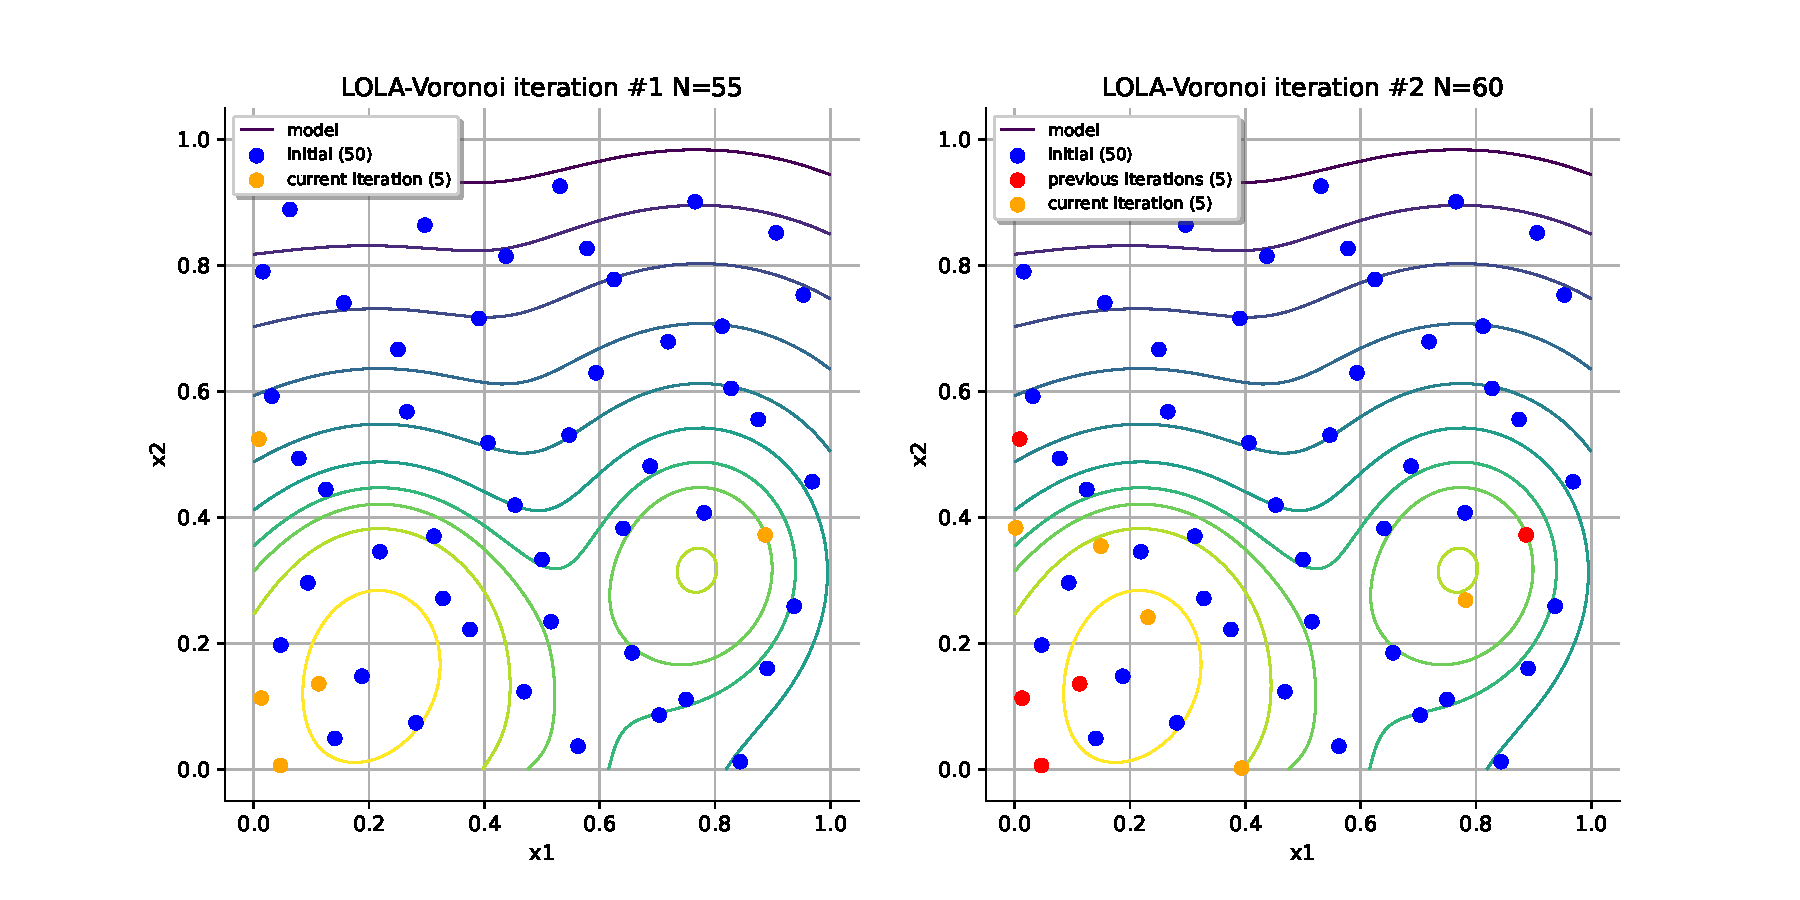
\includegraphics[width=1.0\textwidth]{figures/lolavoronoi_1}
\end{figure}

\end{frame}

%%%%%%%%%%%%%%%%%%%%%%%%%%%%%%%%%%%%%%%%%%%%%%%%%%%%%%%%%%%%%%%%%%%%%%%%%%%%%

\begin{frame}
\frametitle{LOLA-Voronoi sequential design 3/7}

\begin{figure}
   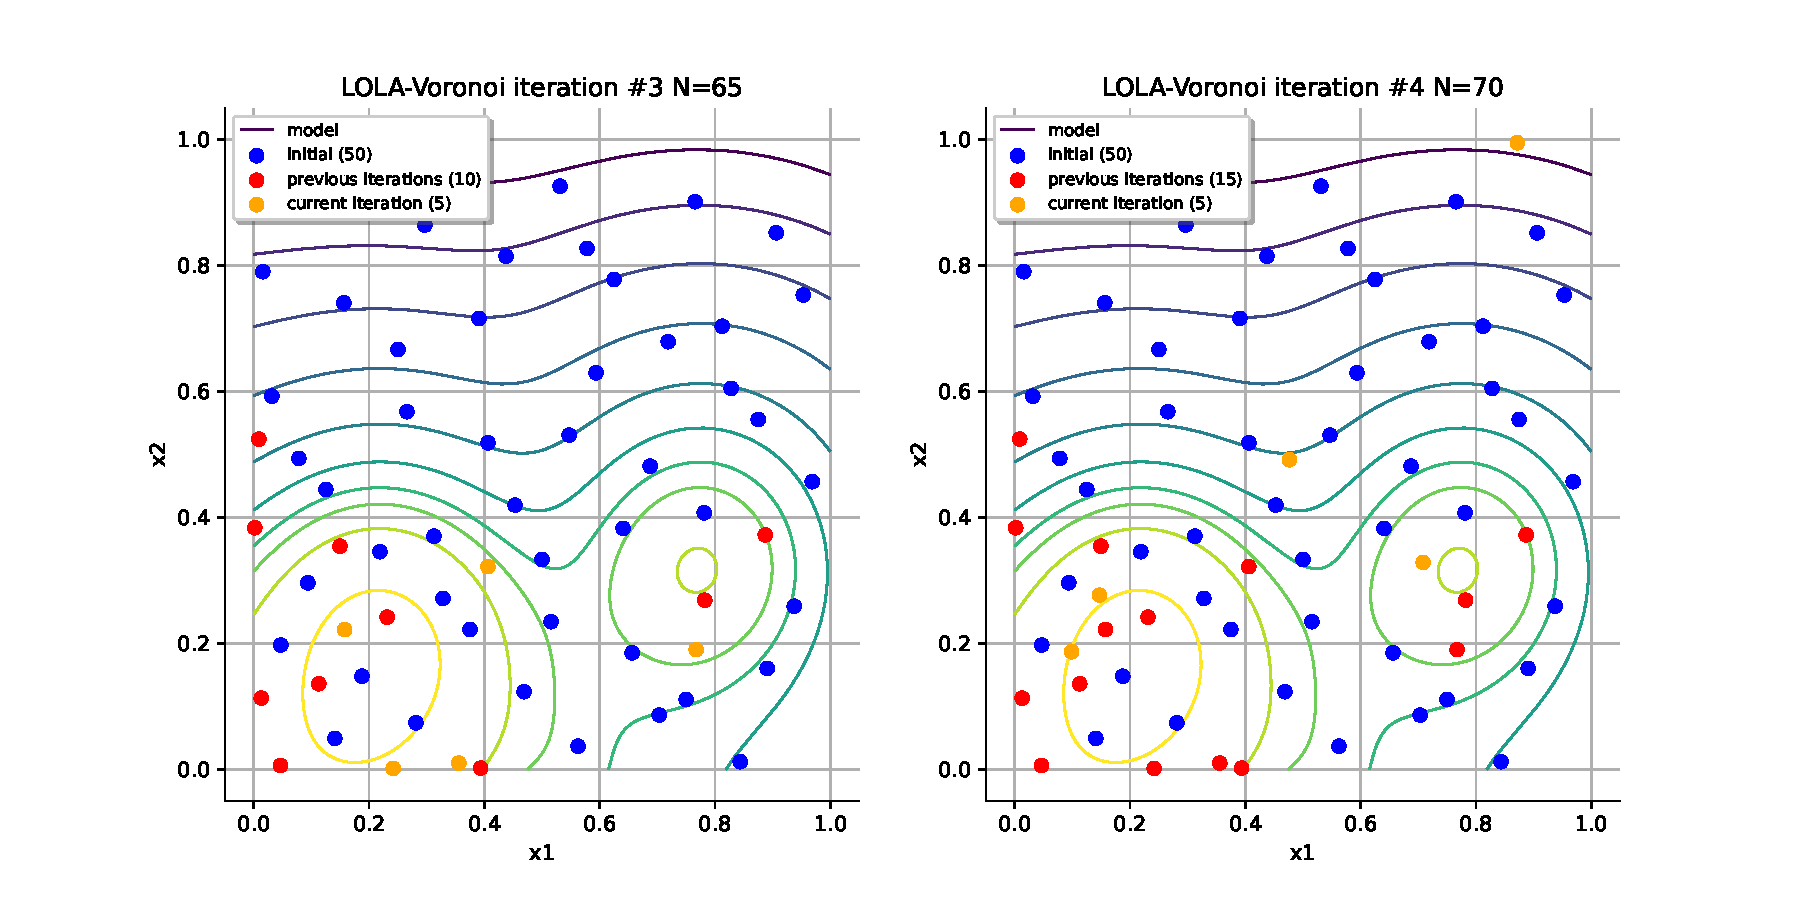
\includegraphics[width=1.0\textwidth]{figures/lolavoronoi_2}
\end{figure}

\end{frame}

%%%%%%%%%%%%%%%%%%%%%%%%%%%%%%%%%%%%%%%%%%%%%%%%%%%%%%%%%%%%%%%%%%%%%%%%%%%%%

\begin{frame}
\frametitle{LOLA-Voronoi sequential design 4/7}

\begin{figure}
   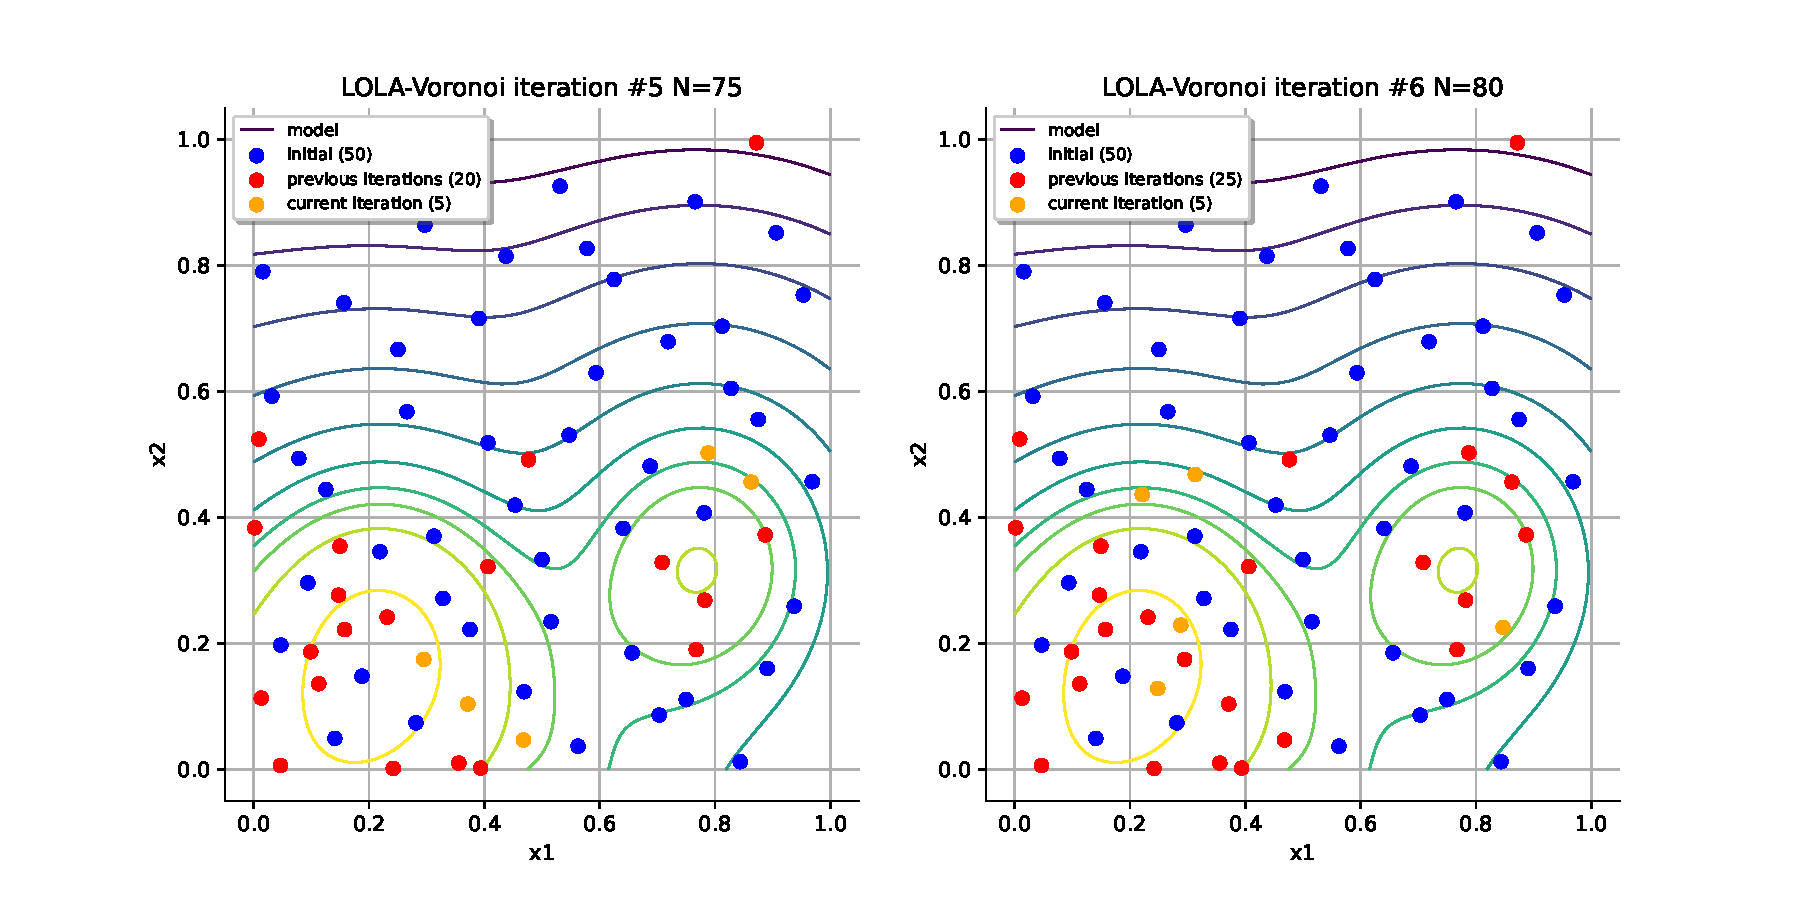
\includegraphics[width=1.0\textwidth]{figures/lolavoronoi_3}
\end{figure}

\end{frame}

%%%%%%%%%%%%%%%%%%%%%%%%%%%%%%%%%%%%%%%%%%%%%%%%%%%%%%%%%%%%%%%%%%%%%%%%%%%%%

\begin{frame}
\frametitle{LOLA-Voronoi sequential design 5/7}

\begin{figure}
   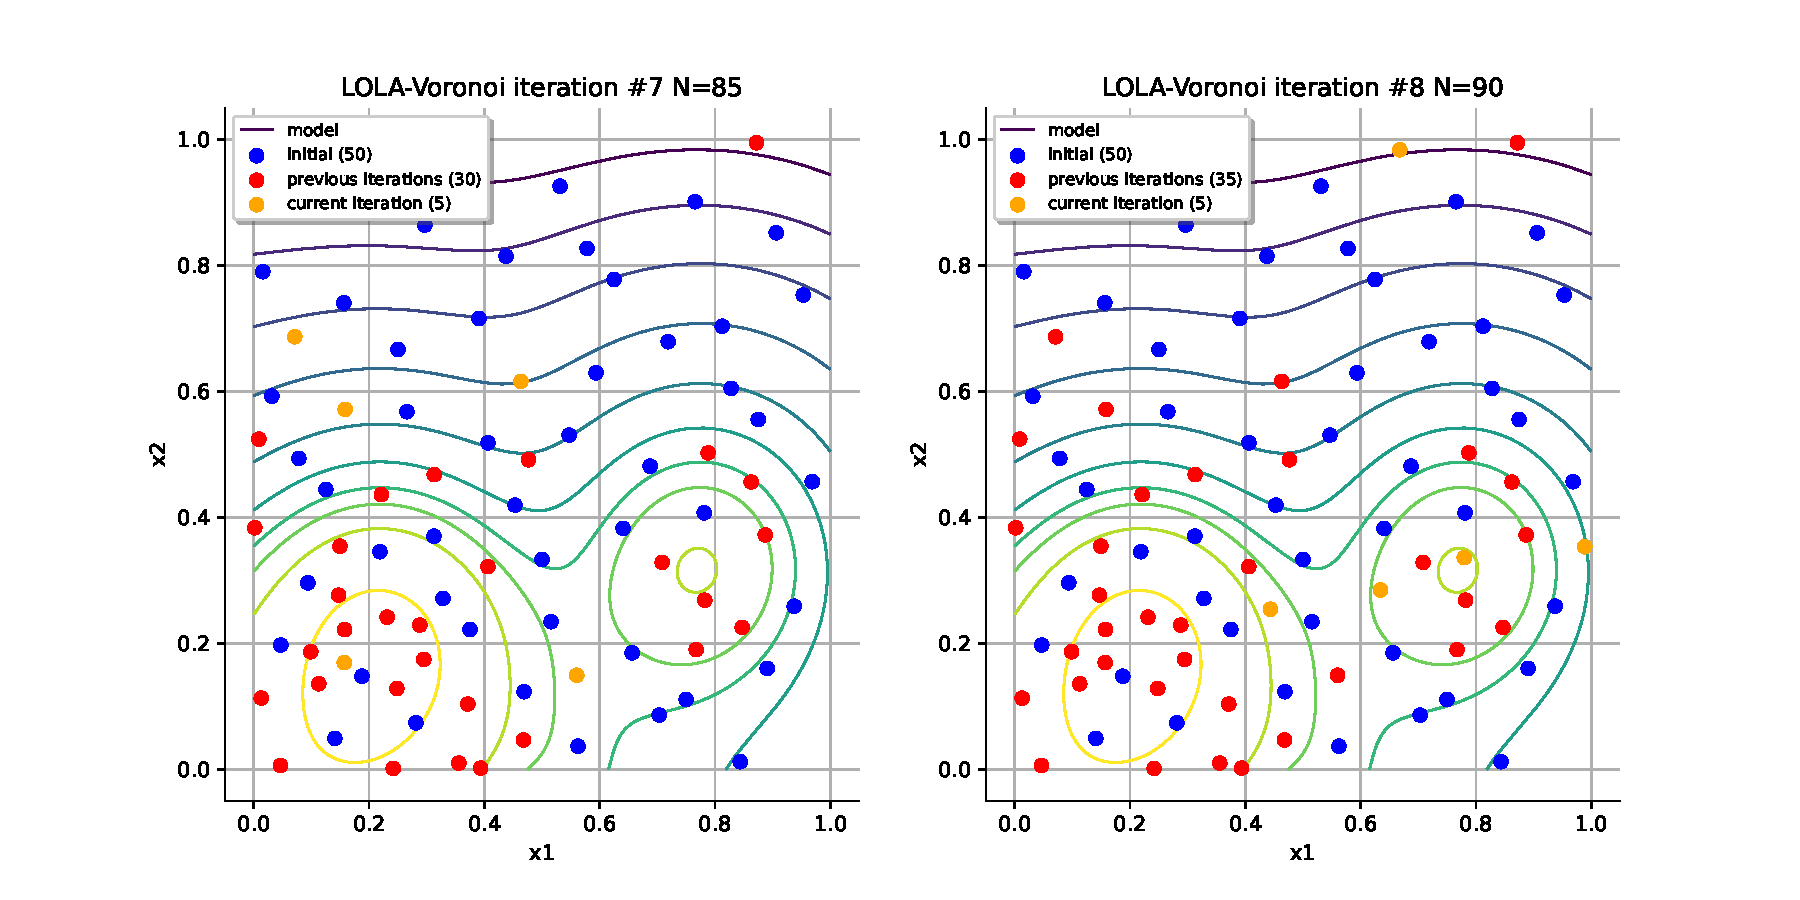
\includegraphics[width=1.0\textwidth]{figures/lolavoronoi_4}
\end{figure}

\end{frame}


%%%%%%%%%%%%%%%%%%%%%%%%%%%%%%%%%%%%%%%%%%%%%%%%%%%%%%%%%%%%%%%%%%%%%%%%%%%%%

\begin{frame}
\frametitle{LOLA-Voronoi sequential design 6/7}

\begin{figure}
   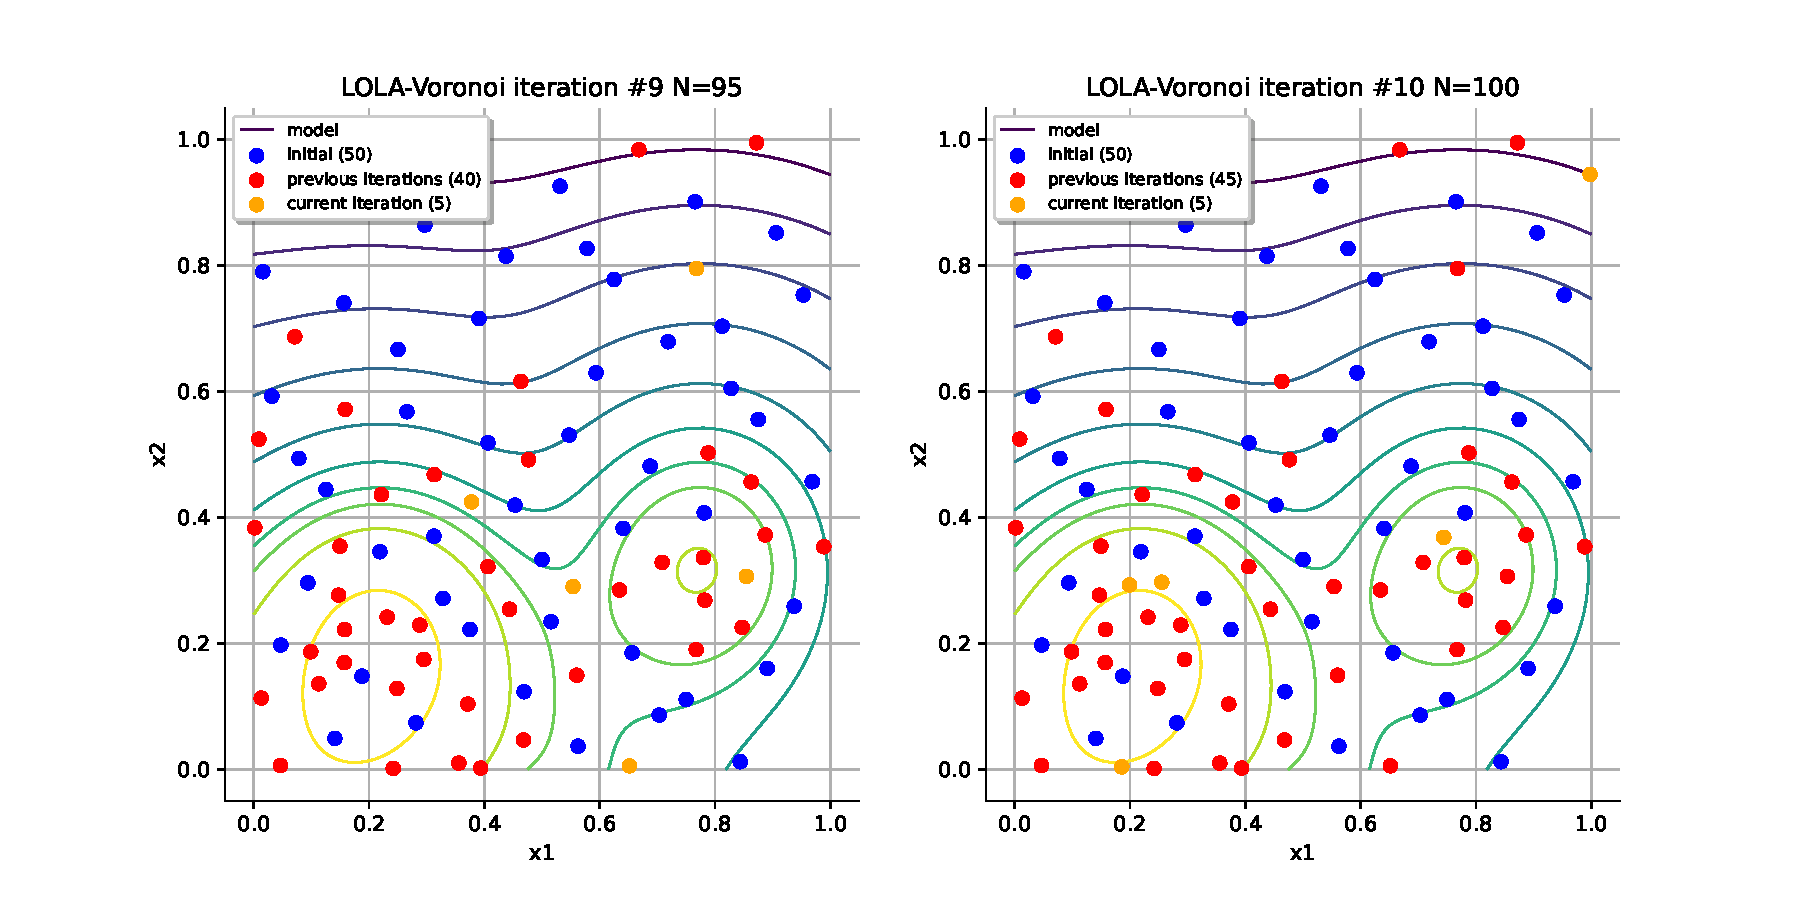
\includegraphics[width=1.0\textwidth]{figures/lolavoronoi_5}
\end{figure}

\end{frame}

%%%%%%%%%%%%%%%%%%%%%%%%%%%%%%%%%%%%%%%%%%%%%%%%%%%%%%%%%%%%%%%%%%%%%%%%%%%%%

\begin{frame}[containsverbatim]
\frametitle{LOLA-Voronoi sequential design 7/7}

\begin{small}
\lstset{language=python}
\begin{lstlisting}
# 1. initial design
distribution = ot.JointDistribution([ot.Uniform(-1.0, 1.0)] * 2)
N = 50
design = ot.LowDiscrepancyExperiment(ot.HaltonSequence(), distribution, N)
x0 = design.generate()
y0 = f1(x0)

# 2. sequential experiment
algo = otexp.LOLAVoronoi(x0, y0, distribution)
for i in range(10):
    x = algo.generate(5)     # generate 5 new input samples
    y = f(x)                 # evaluate output samples
    algo.update(x, y)        # update state with new x/y pairs

# 3. learn metamodel on all samples
x_final = algo.getInputSample()
y_final = algo.getOutputSample()
algo_mm = ot.FunctionalChaosAlgorithm(x_final, y_final, distribution)
algo_mm.run()
metamodel = algo_mm.getResult().getMetaModel()
\end{lstlisting}
\end{small}


\end{frame}

%%%%%%%%%%%%%%%%%%%%%%%%%%%%%%%%%%%%%%%%%%%%%%%%%%%%%%%%%%%%%%%%%%%%%%%%%%%%%

\begin{frame}[containsverbatim]
\frametitle{LeastSquaresEquationsSolver}

Least squares solver for the resolution of a system of non-linear equations.

% \begin{itemize}
% \item Method of moments for initialization
% \item Maximum likelihood for the final estimator
% \end{itemize}

% \begin{figure}
%    
\includegraphics[width=0.4\textwidth]{figures/SmoothedUniformFactory}
% \end{figure}

\begin{small}
\lstset{language=python}
\begin{lstlisting}
import openturns as ot
import openturns.experimental as otexp

inputs = ['x', 'y']
formulas = ['y*x-sin(2*x)', '1 + cos(y) + x']
analytical = ot.SymbolicFunction(inputs, formulas)

algo = otexp.LeastSquaresEquationsSolver()
algo.setResidualError(1e-8)
starting_point = [2.0, 1.0]
solution = algo.solve(analytical, starting_point)
\end{lstlisting}
\end{small}
\end{frame}

%%%%%%%%%%%%%%%%%%%%%%%%%%%%%%%%%%%%%%%%%%%%%%%%%%%%%%%%%%%%%%%%%%%%%%%%%%%%%

% \begin{frame}[containsverbatim]
% \frametitle{Latent variable model}
% 
% \begin{itemize}
% \item Covariance model, for eg Kriging
% \item Covariance between different unordered values (or levels) of a categorical variable
% \item Parameters: coordinates in the latent space
% \item Zhang2020: "A latent variable approach to Gaussian process modeling with qualitative and quantitative factors"
% \end{itemize}
% 
% \vspace{30pt}
% 
% \begin{small}
% \begin{lstlisting}
% import openturns.experimental as otexp
% covModel = otexp.LatentVariableModel(3, 2)
% activeCoordinates = [0.1, 0.3, -0.4]
% covModel.setLatentVariables(activeCoordinates)
% \end{lstlisting}
% \end{small}
% 
% \end{frame}

%%%%%%%%%%%%%%%%%%%%%%%%%%%%%%%%%%%%%%%%%%%%%%%%%%%%%%%%%%%%%%%%%%%%%%%%%%%%%

\section{Metamodelling}

\begin{frame}[containsverbatim]
\frametitle{RatioOfUniforms}
% \begin{itemize}
% \item Vector to field metamodeling and sensitivity using KL + chaos
% \end{itemize}

% \begin{figure}
%    
\includegraphics[width=0.3\textwidth]{figures/sphx_glr_plot_viscous_fall_metamodel_001}
%    
\includegraphics[width=0.3\textwidth]{figures/sphx_glr_plot_viscous_fall_metamodel_002}
%    
\includegraphics[width=0.3\textwidth]{figures/sphx_glr_plot_viscous_fall_metamodel_003}
% \end{figure}

\begin{small}
\begin{lstlisting}
import openturns as ot
import openturns.experimental as otexp
from math import pi

f = ot.SymbolicFunction('x', '(1.5+sin(x))*exp(x)')
log_UnscaledPDF = ot.ComposedFunction(ot.SymbolicFunction('x', 'log(x)'), f)
range_PDF = ot.Interval(0.0, 2.0 * pi)
ratioOfU = otexp.RatioOfUniforms(log_UnscaledPDF, range_PDF, False)
collMultiStart = ratioOfU.initialize()
x = ratioOfU.getRealization()
sample = ratioOfU.getSample(10)
ratioOfU = otexp.RatioOfUniforms(ot.Student(8.5, 3))
\end{lstlisting}
\end{small}


\end{frame}



%%%%%%%%%%%%%%%%%%%%%%%%%%%%%%%%%%%%%%%%%%%%%%%%%%%%%%%%%%%%%%%%%%%%%%%%%%%%%

% \section{Sensitivity}
% 
% \begin{frame}[containsverbatim]
% \frametitle{Rank-based Sobol' indices}
% 
% \begin{itemize}
% \item Data-driven (no need for dedicated design of experiments, just iid design)
% \item Only first-order indices
% \item Gamboa2022: "Global sensitivity analysis: A novel generation of mighty estimators based on rank statistics"
% \end{itemize}
% 
% % \begin{figure}
% %    
\includegraphics[width=0.3\textwidth]{figures/sphx_glr_plot_sensitivity_rank_sobol_001}
% % \end{figure}
% 
% \begin{small}
% \begin{lstlisting}
% X = distributionX.getSample(N)
% Y = f(X)
% algo = otexp.RankSobolSensitivityAlgorithm(X, Y)
% s1 = algo.getFirstOrderIndices()
% \end{lstlisting}
% \end{small}
% 
% \end{frame}

%%%%%%%%%%%%%%%%%%%%%%%%%%%%%%%%%%%%%%%%%%%%%%%%%%%%%%%%%%%%%%%%%%%%%%%%%%%%%

\section{Misc}

\begin{frame}
\frametitle{Documentation improvements}
\begin{itemize}
\item Improved functions API with graphs
\item Improved documentation of Directional sampling classes
\end{itemize}

% \begin{center}
% 
\includegraphics[width=0.3\textwidth]{figures/stiffened_panel_simulation}
% \end{center}

\begin{itemize}
\item Lot of time invested in the improvement of the documentation
\item Consistency of examples
\item SVG graphics
\end{itemize}
\end{frame}

%%%%%%%%%%%%%%%%%%%%%%%%%%%%%%%%%%%%%%%%%%%%%%%%%%%%%%%%%%%%%%%%%%%%%%%%%%%%%

\begin{frame}
\frametitle{Other improvements}
\begin{itemize}
\item Smolyak nested tensorization
\item Advanced validation of Distribution classes
\item Allow MultiStart optimization in FORM algorithms
\end{itemize}

\vspace{6pt}

% \begin{center}
% 
\includegraphics[width=0.15\textwidth]{figures/bugfix}
% \end{center}

\end{frame}

%%%%%%%%%%%%%%%%%%%%%%%%%%%%%%%%%%%%%%%%%%%%%%%%%%%%%%%%%%%%%%%%%%%%%%%%%%%

\begin{frame}
\frametitle{Packaging 1/2}
\begin{block}{Python channels}
\begin{itemize}
\item Pip / Conda
\item Versions: 3.9+
\item OS: Windows, Linux, MacOS
\item Architectures: x86\_64, arm64 (Linux+MacOS)
\end{itemize}
\end{block}

% \begin{figure}
%    
\includegraphics[width=0.3\textwidth]{figures/PyPI_logo}
%    
\includegraphics[width=0.3\textwidth]{figures/Conda_logo.svg}
% \end{figure}

\end{frame}

\begin{frame}
\frametitle{Packaging 2/2}
\begin{block}{Supported Linux distributions}
\begin{itemize}
\item Ubuntu 22/24/25
\item Debian 11/12
\item Fedora 41/42
\item OpenSUSE 15.6
\item Mageia 9
\item ArchLinux
\end{itemize}

... and FreeBSD

\end{block}


\begin{center}

\includegraphics[width=0.05\textwidth]{figures/debian-openlogo-100}

\includegraphics[width=0.08\textwidth]{figures/ubuntu}

\includegraphics[width=0.08\textwidth]{figures/Fedora-Logo}
% 
\includegraphics[width=0.08\textwidth]{figures/centos-logo}

\includegraphics[width=0.08\textwidth]{figures/opensuse-logo}

\includegraphics[width=0.15\textwidth]{figures/200px-Logo_mageia_official}

\includegraphics[width=0.15\textwidth]{figures/archlinux-logo}

\includegraphics[width=0.15\textwidth]{figures/FREEBSD_Logo_Horiz_Pos_RGB}
\end{center}

\end{frame}

%%%%%%%%%%%%%%%%%%%%%%%%%%%%%%%%%%%%%%%%%%%%%%%%%%%%%%%%%%%%%%%%%%%%%%%%%%%

\begin{frame}
\frametitle{Outlook}
\begin{block}{2025-2026 work}
\begin{itemize}
\item Work on functional chaos expansion API
\item Dimension reduction models
\item Interfacing with SMT2 surrogate model toolbox
\item Classification with random forests
\item Calibration with bounds, fonctional models, ABC bayesian method
\item LMG sensitivity indices (dependent variables for linear models)
\item VonMises-Fisher distribution in high dimension, tensorized covariance models
\item Performance of conditioned GP on a large grid
\end{itemize}
\end{block}
\end{frame}

%%%%%%%%%%%%%%%%%%%%%%%%%%%%%%%%%%%%%%%%%%%%%%%%%%%%%%%%%%%%%%%%%%%%%%%%%%%%%

\begin{frame}
\frametitle{Community}

Join our forum: https://openturns.discourse.group


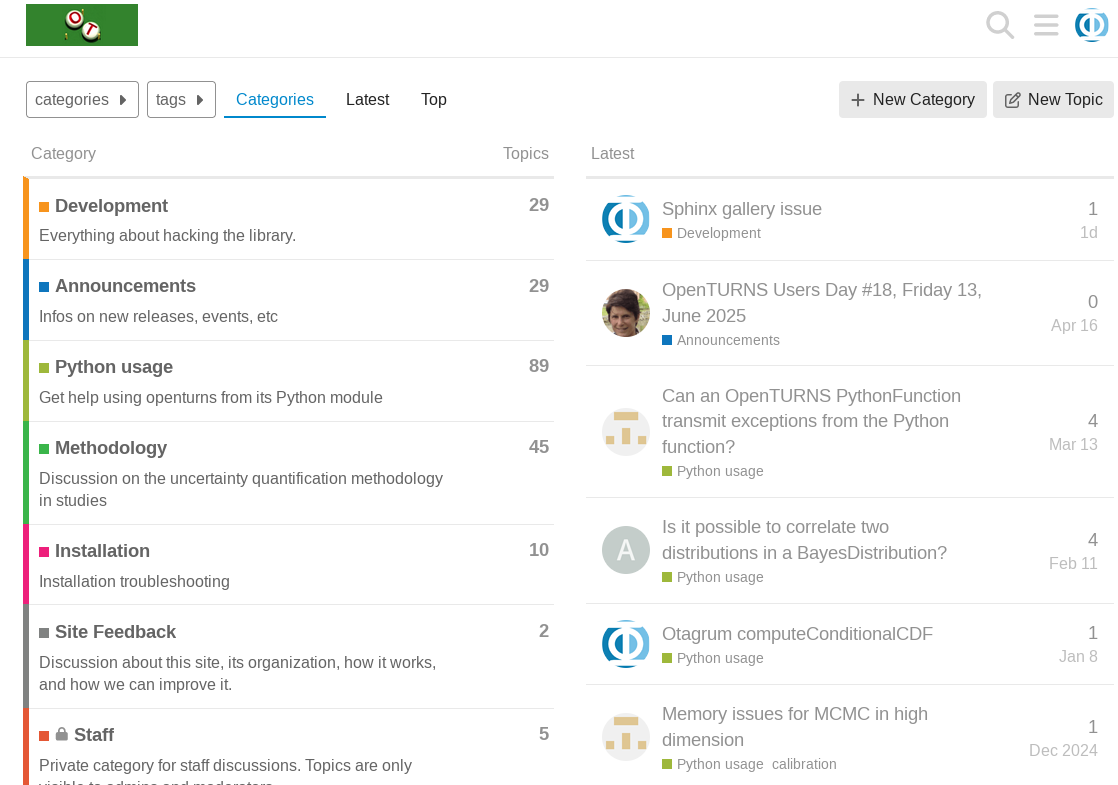
\includegraphics[width=1.0\textwidth]{figures/forum}


% \begin{itemize}
% \item Smolyak nested tensorization
% \item Automatic testing of Distribution services
% \end{itemize}
% 
% \vspace{6pt}

% \begin{center}
% 
\includegraphics[width=0.15\textwidth]{figures/bugfix}
% \end{center}

\end{frame}

%%%%%%%%%%%%%%%%%%%%%%%%%%%%%%%%%%%%%%%%%%%%%%%%%%%%%%%%%%%%%%%%%%%%%%%%%%%%%

\begin{frame}
\frametitle{END}

Thank you for your attention!

Any questions?

\begin{center}
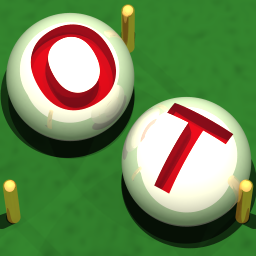
\includegraphics[width=0.2\textwidth]{figures/logo-ot-small}
\end{center}

\end{frame}

% %%%%%%%%%%%%%%%%%%%%%%%%%%%%%%%%%%%%%%%%%%%%%%%%%%%%%%%%%%%%%%%%%%%%%%%%%%%%%
% 
% \section{Bibliography}
% 
% \begin{frame}
% \frametitle{Bibliography}
% 
% \begin{itemize}
% \item Airbus, EDF, ONERA, Phimeca Engineering, IMACS.
% OpenTURNS, a scientific library usable as a Python module dedicated to the treatment of uncertainties, 
% \url{www.openturns.org}.
% \item Airbus, EDF, Phimeca Engineering, IMACS. Documentation of OpenTURNS, version 1.9. 
% \url{http://openturns.github.io/openturns/1.9/contents.html}
% \item  Michaël Baudin, Anne Dutfoy, Bertrand Iooss, and Anne-Laure Popelin. 
% OpenTURNS: An Industrial Software for Uncertainty Quantification in Simulation, 
% Handbook of Uncertainty Quantification, 
% pages 1-38. Springer International Publishing, 2016
% \end{itemize}
% 
% \end{frame}

\end{document}
